\documentclass[tikz,border=10pt]{standalone}
\usetikzlibrary{arrows.meta, positioning, shapes.geometric, shapes.misc, fit, backgrounds, calc, matrix}

\tikzset{
    >=Latex,
    font=\sffamily\large,
    node distance=1.5cm and 3cm,
    dag_result/.style={
        rectangle, 
        draw=green!70!black, 
        fill=green!15, 
        very thick, 
        minimum width=4.5cm, 
        minimum height=1.5cm, 
        text width=5cm,
        align=center
    },
    dag_lemma/.style={
        rounded rectangle, 
        draw=orange!80!black, 
        fill=yellow!20, 
        very thick, 
        minimum width=4.5cm, 
        minimum height=1.5cm, 
        text width=5cm,
        align=center
    },
    dag_model/.style={
        ellipse, 
        draw=blue!70!black, 
        fill=blue!12, 
        very thick, 
        minimum width=4.5cm, 
        minimum height=1.5cm, 
        text width=4.5cm,
        align=center
    },
    dag_unformalized/.style={
        rectangle, 
        draw=gray!60!black, 
        fill=gray!10, 
        very thick, 
        dashed, 
        minimum width=4.5cm, 
        minimum height=1.5cm, 
        text width=5cm,
        align=center
    },
    dag_conditional/.style={
        rectangle, 
        rounded corners,
        draw=orange!80!black, 
        fill=orange!10, 
        very thick, 
        minimum width=4.5cm, 
        minimum height=1.5cm, 
        text width=5cm,
        align=center
    },
    dag_partial/.style={
        rectangle,
        rounded corners,
        draw=yellow!55!black,
        fill=yellow!10,
        very thick,
        dashed,
        minimum width=4.5cm,
        minimum height=1.5cm,
        text width=5cm,
        align=center
    },
    dag_scaffold/.style={
        rectangle,
        draw=gray!55!black,
        fill=white,
        very thick,
        dotted,
        minimum width=4.5cm,
        minimum height=1.5cm,
        text width=5cm,
        align=center
    },
    dag_caveat/.style={
        diamond, 
        draw=red!70!black, 
        fill=red!10, 
        minimum width=4cm, 
        align=center, 
        inner sep=0pt, 
        font=\sffamily\small
    },
    dag_arrow/.style={
        -{Stealth[scale=1.2]}, 
        very thick,
        shorten >=1.5pt,
        shorten <=1.5pt
    },
    dag_dashed_arrow/.style={
        -{Stealth[scale=1.2]}, 
        very thick, 
        dashed,
        shorten >=1.5pt,
        shorten <=1.5pt
    },
    dag_template_legend/.style={
        minimum width=2.6cm,
        minimum height=0.8cm,
        text width=2.45cm,
        inner sep=3pt,
        font=\sffamily\small,
        align=center
    },
    dag_template_note/.style={
        rectangle,
        draw=gray!50,
        fill=gray!5,
        rounded corners,
        text width=13cm,
        align=left,
        font=\sffamily\small,
        inner sep=6pt
    }
}

% Legend Helper
\newcommand{\daglegend}[2]{
    \node[draw, rounded corners, very thick, fit=#1, inner sep=12pt, label=above:\textbf{\Large Legend}] (#2) {};
}


\begin{document}
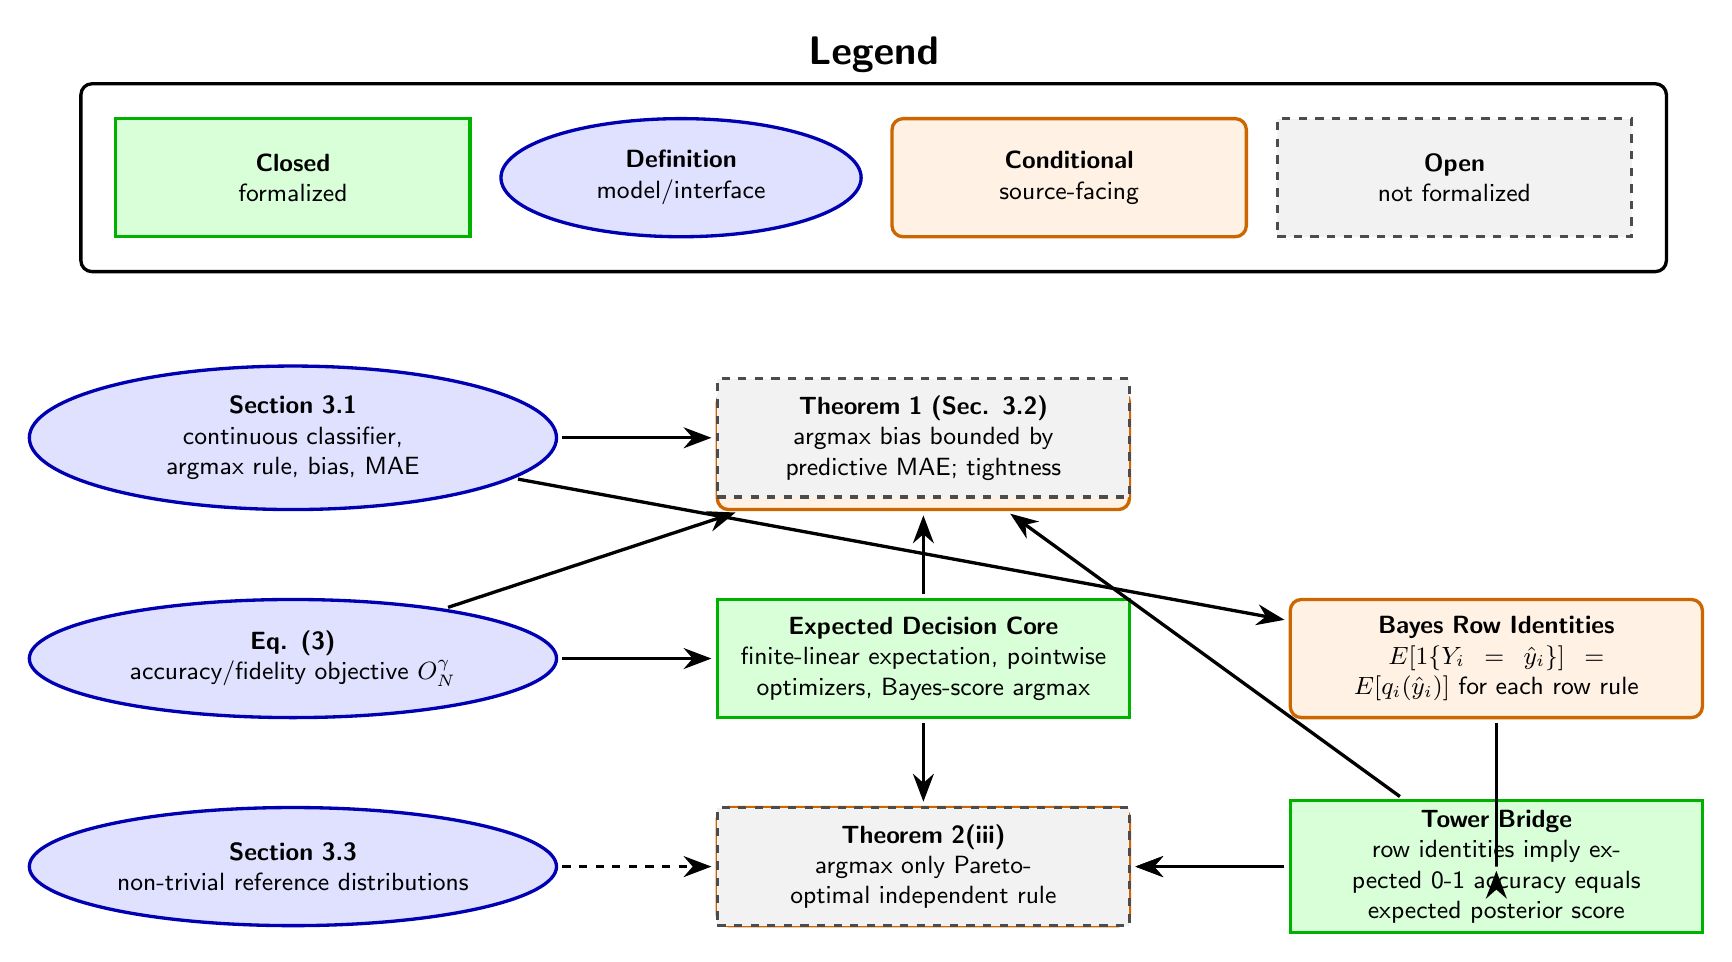
\begin{tikzpicture}[node distance=1.1cm and 2cm,
  every node/.style={font=\sffamily\small}]

% Legend
\node[dag_result, text width=3cm] (legRes) {\textbf{Closed}\\formalized};
\node[dag_model, right=0.35cm of legRes, text width=3cm] (legDef) {\textbf{Definition}\\model/interface};
\node[dag_conditional, right=0.35cm of legDef, text width=3cm] (legCond) {\textbf{Conditional}\\source-facing};
\node[dag_unformalized, right=0.35cm of legCond, text width=3cm] (legOpen) {\textbf{Open}\\not formalized};
\daglegend{(legRes)(legDef)(legCond)(legOpen)}{Legend}

% Paper definitions and objectives
\node[dag_model, below=1.6cm of legRes] (Scores)
  {\textbf{Section 3.1}\\continuous classifier, argmax rule, bias, MAE};
\node[dag_model, below=of Scores] (DecisionObj)
  {\textbf{Eq. (3)}\\accuracy/fidelity objective $O_N^\gamma$};
\node[dag_model, below=of DecisionObj] (Nontrivial)
  {\textbf{Section 3.3}\\non-trivial reference distributions};

% Current reusable expected-decision layer
\node[dag_result, right=of DecisionObj] (Argmax)
  {\textbf{Expected Decision Core}\\finite-linear expectation, pointwise optimizers, Bayes-score argmax};
\node[dag_conditional, above=of Argmax] (Thm2i)
  {\textbf{Theorem 2(i)}\\joint rule maximizes $O_N^\gamma$ assuming row Bayes identities};
\node[dag_conditional, below=of Argmax] (Thm2ii)
  {\textbf{Theorem 2(ii)}\\argmax maximizes expected accuracy assuming row Bayes identities};

% Source theorems
\node[dag_unformalized, right=of Scores] (Thm1)
  {\textbf{Theorem 1 (Sec. 3.2)}\\argmax bias bounded by predictive MAE; tightness};
\node[dag_unformalized, right=of Nontrivial] (Thm2iii)
  {\textbf{Theorem 2(iii)}\\argmax only Pareto-optimal independent rule};
\node[dag_conditional, right=of Argmax] (RowBayes)
  {\textbf{Bayes Row Identities}\\$E[1\{Y_i=\hat y_i\}] = E[q_i(\hat y_i)]$ for each row rule};
\node[dag_result, right=of Thm2ii] (BayesBridge)
  {\textbf{Tower Bridge}\\row identities imply expected 0-1 accuracy equals expected posterior score};

% Edges
\draw[dag_arrow] (Scores) -- (Thm1);
\draw[dag_arrow] (DecisionObj) -- (Argmax);
\draw[dag_arrow] (Argmax) -- (Thm2i);
\draw[dag_arrow] (Argmax) -- (Thm2ii);
\draw[dag_arrow] (DecisionObj) -- (Thm2i);
\draw[dag_arrow] (Scores) -- (RowBayes);
\draw[dag_arrow] (RowBayes) |- (BayesBridge);
\draw[dag_arrow] (BayesBridge) -- (Thm2ii);
\draw[dag_arrow] (BayesBridge) -- (Thm2i);
\draw[dag_dashed_arrow] (Nontrivial) -- (Thm2iii);
\draw[dag_dashed_arrow] (BayesBridge) -- (Thm2iii);

\end{tikzpicture}
\end{document}
